% Derived from projects/eos/trunk/coda14.tex Documetnation for poster
% mode at
% http://http://nxg.me.uk/dist/textpos/textpos.pdf

\newcommand\cf{c_f}
\newcommand{\vol}{v}
\newcommand{\eos}{f}
\newcommand{\eosnom}{\tilde f}
\newcommand{\argmin}{\operatorname*{argmin}}
\newcommand{\argmax}{\operatorname*{argmax}}
\newcommand{\normal}[2]{{\cal N}(#1,#2)}
\newcommand{\COST}{\cal C}
\newcommand{\LL}{{\cal L}}
\newcommand{\Prob}{\text{Prob}}
\newcommand{\field}[1]{\mathbb{#1}}
\newcommand{\EV}[2]{\field{E}_{#1}\left[#2\right]}
\newcommand{\nomf}{\tilde f}
\newcommand{\partialfixed}[3]{\left. \frac{\partial #1}{\partial #2}\right|_#3}
\newcommand\CJ[1]{{{#1}_{\text{CJ}}}}
\newcommand\fisher{\mathcal{I}}

\newcommand{\plotsize}{\tiny} % Size of font in labels
%\documentclass[a0,showboxes]{a0poster}
\documentclass[a0]{a0poster}
\usepackage{amsmath}
\usepackage{amsfonts}
%\usepackage{graphix}
\pagestyle{empty}
\setcounter{secnumdepth}{0}

% The textpos package is necessary to position textblocks at arbitary 
% places on the page.
\usepackage[absolute]{textpos}

% Graphics to include graphics. Times is nice on posters, but you
% might want to switch it off and go for CMR fonts.
%\usepackage{graphics,wrapfig,times}
\usepackage[pdftex]{rotating} %AMF

% These colours are tried and tested for titles and headers. Don't
% over use color!
\usepackage{color}
%\definecolor{DarkBlue}{rgb}{0.1,0.1,0.5}
\definecolor{DarkBlue}{rgb}{0.1,0.1,0.8}
\definecolor{Red}{rgb}{0.9,0.0,0.1}

% see documentation for a0poster class for the size options here
\let\Textsize\normalsize
\def\Head#1{\noindent\hbox to \hsize{\hfil{\LARGE\color{DarkBlue} #1}}\bigskip}
\def\LHead#1{\noindent{\LARGE\color{DarkBlue} #1}\bigskip}
\def\Subhead#1{\noindent{\large\color{DarkBlue} #1}\bigskip}
\def\Title#1{\noindent{\VeryHuge\color{Red} #1}}

\TPGrid[40mm,40mm]{23}{12}      % 4 cols of width 5, plus 3 gaps

\parindent=0pt
\parskip=0.5\baselineskip

\begin{document}

% Understanding textblocks is the key to being able to do a poster in
% LaTeX. In
%
%    \begin{textblock}{wid}(x,y)
%    ...
%    \end{textblock}
%
% the first argument gives the block width in units of the grid
% cells specified above in \TPGrid; the second gives the (x,y)
% position on the grid, with the y axis pointing down.

\begin{textblock}{23}(0,0) \Title{Functional UNcertainty Constrained
    by Law and Experiment (F \underline{U.N.C.L.E.})}
\end{textblock}
\begin{textblock}{2}(21,0)
  \begin{center}
    \resizebox{0.7\textwidth}{!}{\includegraphics{figs/authors.jpg}}
  \end{center}
\end{textblock}

\begin{textblock}{2}(0,12)
\Subhead{LA-UR-16-24568}
\end{textblock}

\begin{textblock}{12}(0.2,0.5)
\LHead{Andrew M.~Fraser and Stephen A.~Andrews, Los Alamos National Laboratory}
\end{textblock}

%%%%%%%%%%%%%%%%%Left Hand Column on General Method%%%%%%%%%%%%%%
\begin{textblock}{6}(0,1.25) \LHead{$2^{\text{nd}}$ Order
    Approximation of Log Probability}

  Numerically find MAP estimate parameters of unknown function.  For
  each experiment, estimate the Fisher information $(\fisher_k)$ and
  interpret it as how the $k^\text{th}$ constrains the unknown
  function.
\end{textblock}

\begin{textblock}{6}(0, 2.5)
  \begin{description}
  \item[Experiments] $x=[x_0,\ldots,x_n]$, where $x_k$ is data from
    the $k^\text{th}$ experiment
  \item[Likelihood]
    \begin{equation*}
      p_l(x|\theta) = \prod_k p_l(x_k|\theta)
    \end{equation*}
  \item[Prior]
    \begin{equation*}
      p_p(\theta)
    \end{equation*}
  \item[A posteriori distribution]
    \begin{equation*}
      p(\theta|x) = \frac{p_l(x|\theta) p_p(\theta)}{\int p_l(x|\phi)
        p_p(\phi) d\phi}
    \end{equation*}
  \item[MAP] Maximum A posteriori Probability
    \begin{equation*}
      \hat \theta \equiv \argmax_{\theta} p(\theta|x)
    \end{equation*}
  \item[Taylor series]
    \begin{align*}
      &\log \left( p(\theta|x) \right) = \log \left( \frac{p_l(x|\hat \theta)
        p_p(\hat \theta)}{\int p_l(x|\phi) p_p(\phi) d\phi} \right) \\
      &\qquad~+ \frac{1}{2}
        \left( \theta - \hat \theta \right)^T \left(
        \frac{d^2 \log\left( p_l(x|\phi) \right) }{d\phi^2} +
        \frac{d^2 \log \left( p_p(\phi) \right) }{d\phi^2} 
        \right)_{\phi=\hat \theta} \left( \theta - \hat \theta
        \right)\\
      &\qquad + R \\
      &\qquad\equiv C + \frac{1}{2}
        \left( \theta - \hat \theta \right)^T H \left( \theta - \hat \theta \right)
        + R
    \end{align*}
  \item[Gaussian approximation]
    \begin{align*}
      \theta|x &\sim {{\cal N}\left( \hat \theta,\Sigma = H^{-1} \right)}\\
      p(\theta|x) &= \frac{1}{\sqrt{(2\pi)^{\text{dim}}|\Sigma|}} \exp\left(
                    -\frac{1}{2}(\theta-\hat\theta)^\mathrm{T}\Sigma^{-1}
                    (\theta-\hat\theta) \right)
    \end{align*}
  \item[Fisher information]
    $\fisher_k \equiv -
    \EV{X_k}{\left[\left. \frac{\partial^2}{\partial\theta^2} \log
          p(X_k;\theta)\right|\theta \right]}$
  \end{description}
  % \vspace{2cm}
  % \begin{center}
  %   \vspace{2cm}
  %   \resizebox{0.3\textwidth}{!}{\includegraphics{authors.jpg}} \\
  %   Photograph of the authors
  % \end{center}
\end{textblock}
\begin{textblock}{6}(0,8.7)
  \LHead{Bibliography}
  
  Andersen, M. and Vandenberghe, L.. ``cvxopt\: Convex Optimization
  Package'' http://cvxopt.org

  Ficket, W. and Davis, W. C., 2000. ``Detonation''. University of
  California Press: Berkeley, CA.

  ``F\_UNCLE: Functional Uncertainty Constrained by Law and Experiment''.\\
  LA-CC-16-034, Los Alamos National Laboratory,
  https://github.com/fraserphysics/F\_UNCLE
  
  Hixson, R. S. et al., 2000. ``Release isentropes of overdriven
  plastic-bonded explosive PBX-9501''  \emph{J. Applied Physics}
  \textbf{88} (11) pp. 6287-6293

  Jones, E., Oliphant, E., Peterson, P., et al. ``SciPy\: Open Source
  Scientific Tools for Python'', 2001-, http://www.scipy.org
  
  Pemberton et al. ``Test Report for Equation of State Measurements of
  PBX-9501''. LA-UR-11-04999, Los Alamos National Laboratory, Los
  Alamos, NM.

  % van der Walt, S. , Colbert, C. S.  and Varoquaux, G.. "The NumPy
  % Array\: A Structure for Efficient Numerical Computation", Computing
  % in Science \& Engineering, \textbf{13}, 22-30 (2011),
  % `DOI:10.1109/MCSE.2011.37 <https://doi.org/10.1109/MCSE.2011.37>`

  % Vaughan, D. E. and Preston, D. L. "Physical Uncertainty Bounds
  % (PUB)". LA-UR-14-20441, Los Alamos National Laboratory, Los Alamos,
  % NM.

  % Hunter, J. D.. "Matplotlib\: A 2D Graphics Environment", Computing
  % in Science \& Engineering, \textbf{9}, 90-95 (2007),
  % `DOI:10.1109/MCSE.2007.55 <https://doi.org/10.1109/MCSE.2007.55>`
\end{textblock}
\newcommand\colB{7}
\newcommand\colC{11}
\newcommand\colD{15}
\newcommand\colE{19}
%%%%%%%%%Upper Right Row on EOS%%%%%%%%%%%%%%%%%%%%%%%%%%%%%%%%%%
\newcommand\EOSY{1.3}
\begin{textblock}{4}(\colB,\EOSY)
  \LHead{Unknown EOS function}

  \resizebox{0.9\textwidth}{!}{\includegraphics{figs/eos_nom_true.pdf}}\\
\end{textblock}
\begin{textblock}{3.7}(\colC,\EOSY)
  \begin{description}
  \item[Pressure] unknown function, $p(\vol)$
  \item[Spline] Represent functions as cubic splines with fixed knot
    locations.  Optimize over coefficients.
  \item[Prior] Gaussian with mean coefficients, $\cf[i]$, fit to
    \begin{equation*}
      \eosnom(\vol) = \frac{F}{\vol^3}, \text{ where } F \leftrightarrow
      2.56\times10^9 \text{Pa} \text{ at one cm}^{3}\text{g}^{-1}
    \end{equation*}
    and variance
    \begin{equation*}
      \sigma^2[i] = \left( 0.05 \cdot\cf[i] \right)^2
    \end{equation*}

  \item[Constraints] Enforced by CVXOPT, (Not consistent with prior)
    \begin{itemize}
    \item Positive
    \item Monotonic
    \item Convex
    \end{itemize}
  \end{description}
\end{textblock}
\begin{textblock}{4}(\colD,\EOSY)
  \begin{center}
    \resizebox{0.7\textwidth}{!}{\includegraphics{figs/basis.pdf}} \\
    Cubic spline basis functions with first and second derivatives.
  \end{center}
\end{textblock}
\begin{textblock}{4}(\colE,\EOSY)
  \vspace{2cm}
  \begin{center}
  \resizebox{0.9\textwidth}{!}{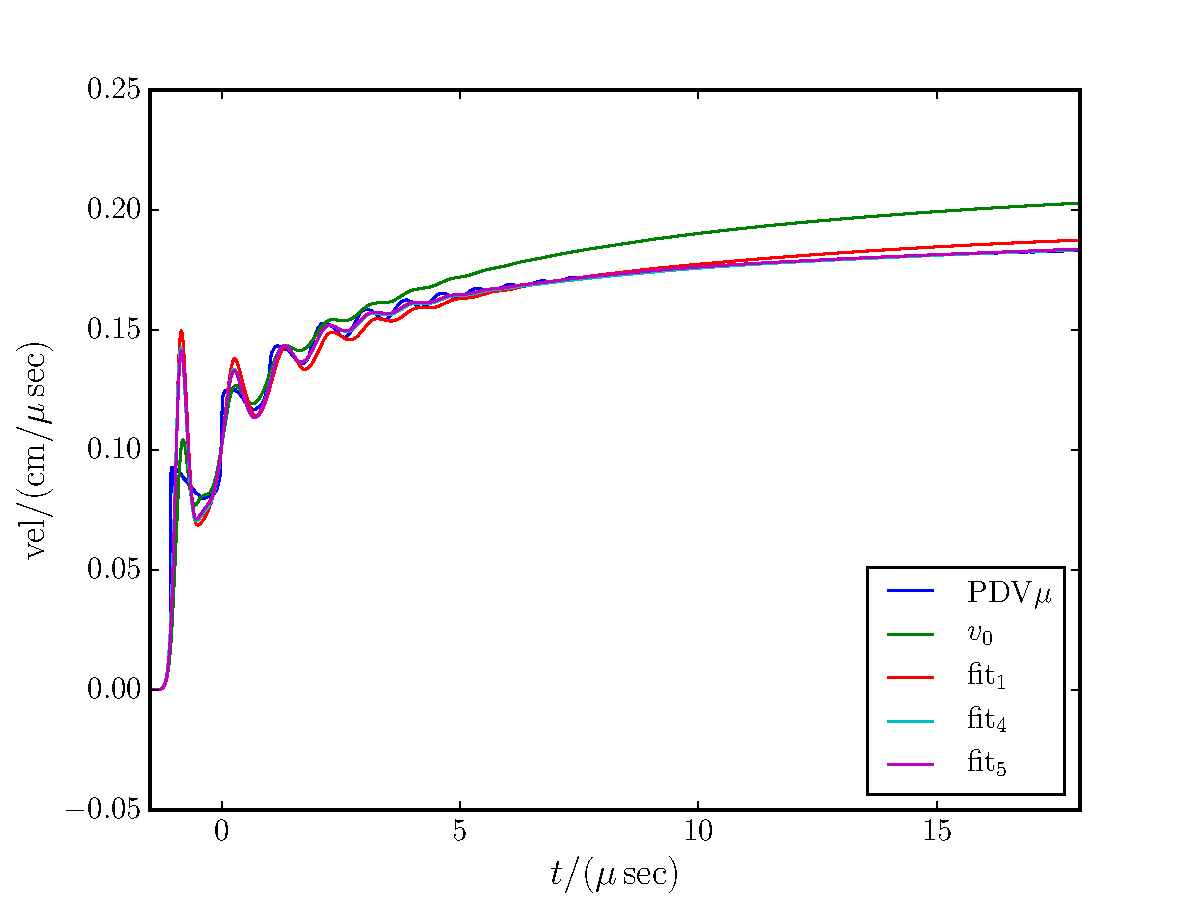
\includegraphics{figs/real.pdf}}\\
  Photon Doppler velocimetry (PDV) data and sequence of fits to
  experiments on PBX-9501.
  \end{center}
\end{textblock}

%%%%%%%%%Upper Right Row on Rate Stick%%%%%%%%%%%%%%%%%%%%%%%%%%%
\newcommand\StickY{5}
\begin{textblock}{4}(\colB,\StickY)
  \LHead{Rate Stick Experiment}\\
  \resizebox{0.9\textwidth}{!}{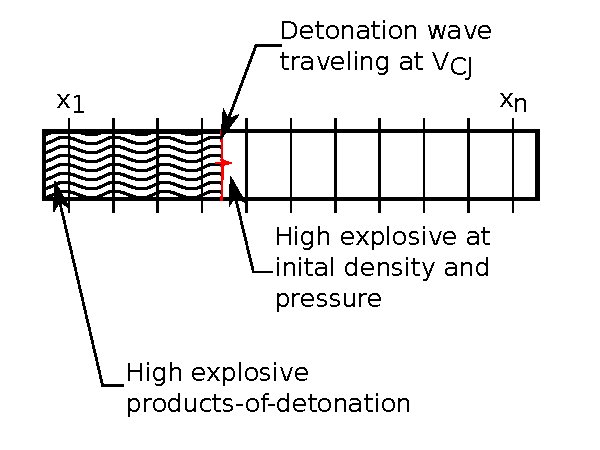
\includegraphics{figs/stick_poster.pdf}}\\
\end{textblock}

\begin{textblock}{4}(\colC,\StickY)
  \resizebox{0.9\textwidth}{!}{\includegraphics{figs/stick_xt.pdf}}\\
\end{textblock}

\begin{textblock}{4}(\colD,\StickY)
  \resizebox{0.9\textwidth}{!}{\includegraphics{figs/stick_CJ.pdf}}\\
  Detonation velocity from Chapman Jouguet conditions:
  \begin{itemize}
  \item \emph{Rayleigh line} through $(v_0, p_0)$ and tangent to EOS
    defines $(\CJ{v}, \CJ{p})$
  \item Velocity $V_\text{CJ} = v_0 \sqrt{\frac{\CJ{p}-p_0}{v_0-\CJ{v}}}$
  \end{itemize}

\end{textblock}

\begin{textblock}{4}(\colE,\StickY)
  \resizebox{0.9\textwidth}{!}{\includegraphics{figs/stick_fisher.pdf}}\\
\end{textblock}

%%%%%%%%Lower Right Row on Gun%%%%%%%%%%%%%%%%%%%%%%%%%%%%%%%%%%%
\newcommand\GunY{9}
\begin{textblock}{4}(\colB,\GunY)
  \LHead{Gun Experiment}\\
  \resizebox{0.9\textwidth}{!}{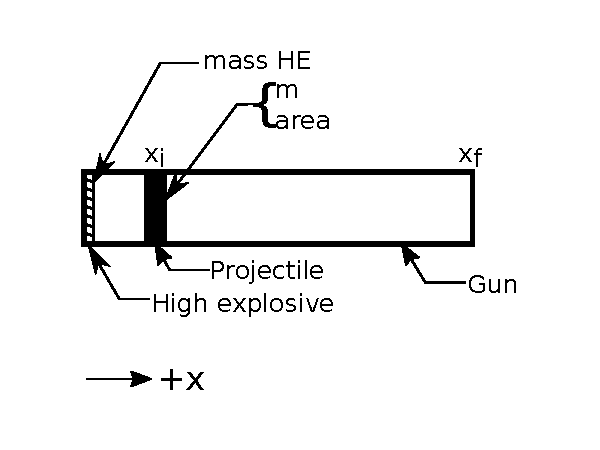
\includegraphics{figs/gun_poster.pdf}}\\
\end{textblock}

\begin{textblock}{3.5}(\colC,\GunY)
  \begin{align*}
    F &= m\cdot a \\
    p(v)\cdot A &= m \cdot \frac{d^2}{d t^2} x \\
    p\left(\frac{A\cdot x}{m_{H.E.}}\right) \frac{A}{m} &= \frac{d^2}{d t^2} x \\
    \begin{bmatrix}
      z_1 \\ z_2
    \end{bmatrix}
      &\equiv 
        \begin{bmatrix}
          x \\ \frac{dx}{dt}
        \end{bmatrix} \equiv 
        \begin{bmatrix}
          x \\ V
        \end{bmatrix} \\
    \frac{dz}{dt} &= \begin{bmatrix}
                      z_2 \\ p(A\cdot z_1) \frac{A}{m}
                    \end{bmatrix}
  \end{align*}
  \begin{itemize}
  \item Sample times
    $\mathbf{t} = [0, \Delta_t, 2 \Delta_t, \cdots, N \Delta_t]$
  \item scipy.integrate.odeint $\rightarrow~[V_0, V_1, \cdots, V_N]$
  \item scipy.interpolate.UnivariateSpline $\rightarrow~V(t)$
  \end{itemize}
  
\end{textblock}

\begin{textblock}{4}(\colD,\GunY)
  \resizebox{0.9\textwidth}{!}{\includegraphics{figs/gun_tv.pdf}}\\
\end{textblock}

\begin{textblock}{4}(\colE,\GunY)
  \resizebox{0.9\textwidth}{!}{\includegraphics{figs/gun_fisher.pdf}}\\
\end{textblock}

\end{document}

%%%---------------
%%% Local Variables:
%%% eval: (TeX-PDF-mode)
%%% End:
